\clearpage
\section{Developed work}
\label{ch:developed}

This section presents the work carried out so far that is assisting the
development of this doctoral research project. \autoref{sec:module} talks about
some available software tools for performance evaluation and presents the new
OpenFlow module for simulations. \autoref{sec:scenario} introduces the proposed
\ac{SDN}-enabled \ac{LTE} simulation scenario, describing its design targets
and the network topology. Finally, \autoref{sec:controller} describes the
enhanced OpenFlow controller for the \ac{SDN}-enabled \ac{LTE} network.
% The work presented here is potential precursor of this doctoral research
% project.


%=============================================================================%
\subsection{The OpenFlow 1.3 module for \acs{ns-3}}
\label{sec:module}

The use of real test beds for experiments in \ac{LTE} networks is typically not
viable, mainly due to high costs of hardware devices and legislation issues
concerning radio spectrum usage. A simple alternative is a software-based
evaluation, including emulation in virtualized environments, and simulations.
\autoref{subsec:softwares} presents some existing software tools that could be
used for evaluation of \ac{SDMN} proposals. The benefits and limitations of
these tools lead to the development of a novel OpenFlow 1.3 simulation module,
which is introduced in \autoref{subsec:ofswitch13}.

%-----------------------------------------------------------------------------%
\subsubsection{Available software tools}
\label{subsec:softwares}

When talking about OpenFlow, the straightforward software tool is
\emph{Mininet}~\cite{Mininet}. It is an open-source emulator that provides a
quick and easy way to prototype and evaluates \ac{SDN} networks. It creates
user-space or kernel full-compliant OpenFlow switches (Open vSwitch), allowing
the use of real controller and software. The virtual network can run real
software, so it can also be used to interactively test networking software.
However, Mininet is a generic tool that models only the switches and links.
\citet{Fontes2015} present Mininet-WiFi, a fork of Mininet extended to support
Wi-Fi by adding virtualized stations and \acp{AP} based on common Linux
wireless device drivers. However, to emulate a complete \ac{LTE} network within
it would require implementing the \ac{E-UTRAN} and \ac{EPC} elements. Moreover,
Mininet suffers from maximum link bandwidth limited by hardware processing
power and no time dilation that prevents it from carrying out emulations when
computational demand is higher than the real-time processing capacity.

A reasonable choice would be using a simulated environment to this end, as the
\emph{\acf{ns-3}}~\cite{ns3}, developed to provide an extensible platform for
networking research and education. This is an open-source discrete event
simulator, designed to work not only with simulations but also with virtualized
test bed environments. It is structured in modules, and among them, there is
the \emph{\ac{LENA}}~\cite{lena}. \ac{LENA} is an open source project that
allows \ac{LTE} small and macro cell vendors to design and test algorithms and
solutions. Target applications for \ac{LENA} include the design and performance
evaluation of downlink and uplink schedulers, radio resource management
algorithms, inter-cell interference coordination, load balancing and mobility
management, \acp{HetNet} solutions, end-to-end \ac{QoE} provisioning, multiple
access network solutions and cognitive \ac{LTE} systems.

Another \ac{ns-3} available module is the \emph{OpenFlow
switch}~\cite{ns3of2010}, which relies on an external OpenFlow switch library
linked to the simulator. This module implements a very outdated protocol
(\citet{ofs089}), and too many new major features were introduced up to the
latest version (\citet{ofs151}). Among these new features, it is possible to
cite multiple tables in the pipeline, group tables, virtual ports, extensible
match support, \acs{IP}v6 support, per flow meters, auxiliary connections,
support for multiple controllers, optical port properties, flow monitoring,
eviction, scheduled bundles, and egress tables. Thus, the available OpenFlow
module does not seem an attractive option for use nowadays.

A possible strategy would be linking \ac{ns-3} and Mininet together,
redirecting \ac{LENA} traffic from the simulator to the emulated OpenFlow
network, but the time dilation constraint in Mininet prevents it, as simulating
large scenarios in \ac{ns-3} may be slower than real time.

%-----------------------------------------------------------------------------%
\subsubsection{The OFSwitch13 module}
\label{subsec:ofswitch13}

The performance evaluation of \ac{SDN} and \ac{LTE} integrated networks was
enumerated in \autoref{subsec:challenges} as one of the open challenges in the
area. To provide a flexible alternative to this limitation, a new
\emph{OpenFlow 1.3 module} was developed for the \ac{ns-3}
simulator~\cite{ofswitch13, Chaves2015}. This module, named
\texttt{OFSwitch13}, uses the external OpenFlow 1.3 software switch
\texttt{ofsoftswitch13}~\cite{ofsoftswich13} linked as a library.
\autoref{fig:ofswitch13-module} illustrates the proposed module.

\begin{figure}[htb]
  \centering
  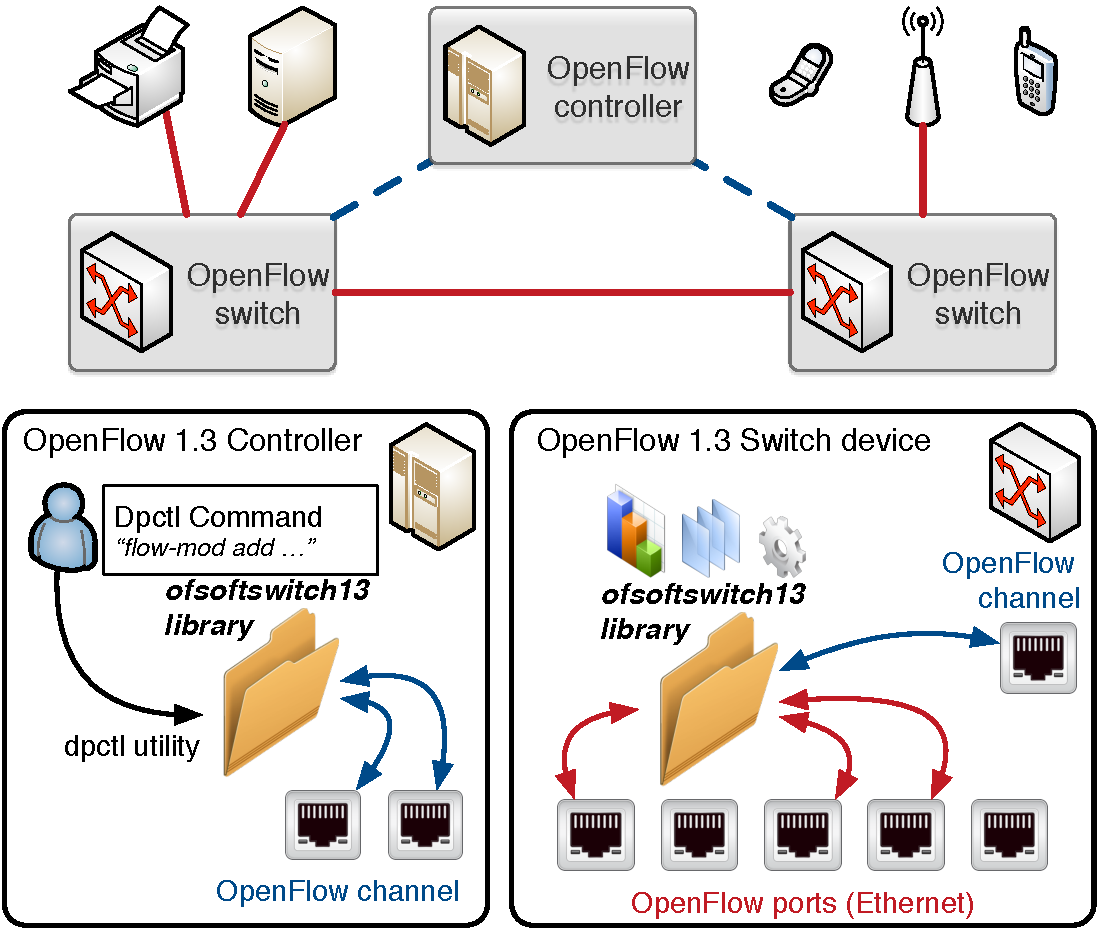
\includegraphics[scale=0.58]{ofswitch13-module}
  \caption{The OpenFlow 1.3 module for \acs{ns-3}.}
  \label{fig:ofswitch13-module}
\end{figure}

The \texttt{OFSwitch13} module interconnects the \ac{ns-3} simulator to the
external \texttt{ofsoftswitch13} library, using its user-space datapath
implementation to create an OpenFlow 1.3 switch device. OpenFlow ports attached
to this device can interconnect with other simulated switches or hosts to send
and receive traffic using standard Ethernet devices available in \ac{ns-3}.
These ports support multiple output queues and internal priority scheduling
mechanism. To orchestrate the switches, an OpenFlow 1.3 controller base class
is also defined, using a dedicated OpenFlow control channel over plain \ac{TCP}
to connect to switches. This generic controller is based on the \texttt{dpctl}
utility, also available in the \texttt{ofsoftswitch13} library. With
\texttt{dpctl}, the developer can use command lines with a simple syntax to
build and send OpenFlow messages to the switches. There is a \emph{Learning
Controller} implementation simulating a learning switch, but the controller can
be extended to implement any complex desired logic. The \texttt{OFSwtich13}
module has currently some limitations: no control channel encryption (\ac{ns-3}
offers no \ac{TLS}), and no support for multiple controllers nor auxiliary
connections. However, the absence of these features does not prevent the use of
its datapath, which is fully functional.

Using this module together with \ac{ns-3} features, it is possible to simulate
not only OpenFlow networks but also from simple to complex \ac{SDN}-enabled
\ac{LTE} networks. As \ac{LENA} provides both \ac{E-UTRAN} and \ac{EPC} models,
including user and control plane, the developer can create specialized
controllers to manage \ac{LTE} networks, and embed OpenFlow switches in
\ac{EPC} elements, for instance. Since \ac{ns-3} is free software, it is
possible to modify the protocols in any desired way to proper integrate both
technologies and evaluate new architectures.


%=============================================================================%
\subsection{\acs{SDN}-enabled \acs{LTE} network}
\label{sec:scenario}

To propose and evaluate new algorithms and protocols for an \ac{SDN}-enabled
\ac{LTE} network, a simulation scenario was created joining \ac{LENA} and
\texttt{OFSwtich13} modules in \ac{ns-3}. First, \autoref{subsec:applications}
shows the adapted \ac{ns-3} applications that are used to generate traffic for
the \ac{LTE} network. Then, \autoref{subsec:design} discusses the scenario
design and topology.

%-----------------------------------------------------------------------------%
\subsubsection{Applications and traffic}
\label{subsec:applications}

\ac{LTE} mobile networks are focused on \ac{VoIP}, multimedia and data
applications over \ac{IP}. To provide a more realistic scenario for
simulations, four different client-server applications were adapted from
existing \ac{ns-3} applications, and are available for use during simulations:
\begin{itemize}
  \item An \emph{\ac{HTTP} application} simulates a client who establishes a
  \ac{TCP} connection with the server and sends a request for the main object
  of a given web page. When the client gets the main object, it process the
  message and start to request the inline objects of the given web page. After
  receiving all inline objects, the client waits a reading time interval before
  requesting a new main object of a new web page. This application was adapted
  from contributions sent to the ns-3-users mailing list, and the traffic model
  used in this application is based on the distributions indicated by
  \citet{Pries2012}.

  \item A \emph{\ac{VoIP} application} simulates a bidirectional \ac{VoIP}
  traffic, encoded with the G.729 codec ($\approx~8.0$~Kbps for payload), and
  sent over \ac{UDP} protocol. The average call length is expected to be 100
  seconds~\cite{Guo2007, Melo2010} and is set by a normal distribution \ac{RNG}
  $\mathcal{N}(100,100)$. This application was adapted from the
  \texttt{OnOffApplication} available in \ac{ns-3}.

  \item A \emph{Live Video Streaming application} simulates a unidirectional
  \ac{UDP} streaming following one trace among a collection of \acs{MPEG}-4
  video trace files presented by~\citet{Fitzek2001}. The average bit rate for a
  trace varies from 100\,Kbps to 1.1\,Mbps, and the file is randomly selected
  by the application. The average video length is expected to be 90
  seconds~\cite{youtubeStats} and is set by a normal distribution \ac{RNG}
  $\mathcal{N}(90,225)$. This application was adapted from the
  \texttt{UdpTraceFile} \ac{ns-3} application.

  \item A \emph{Buffered Video Streaming application} simulates a
  unidirectional \ac{TCP} video streaming, using the same traces from the live
  video streaming application, except that it can buffer the video and send it
  as fast as the network can support. The average video size is calculated to
  match the expected video length for the live streaming application. This
  application is based on the \texttt{BulkSendApplication} and
  \texttt{UdpTraceFile} \ac{ns-3} applications.
\end{itemize}

These four applications are used to provide five different types of traffic
flows in the network, with different \ac{QoS} requirements.
\autoref{tab:applications} shows the \ac{EPS} bearer mapping used for available
applications. Note that the traffic from the live video streaming application
can be sent over \ac{GBR} and Non-\ac{GBR} bearers.

\begin{table}[b!]
  \caption{Bearer \acs{QCI} mapping for applications.}
  \label{tab:applications}
  \centering
  \begin{tabular}{lll}
    \toprule
    \bfseries \acs{QCI} & \bfseries Bearer type & \bfseries Application \\
    \midrule
    1 & \ac{GBR}     & \ac{VoIP} \\
    2 & \ac{GBR}     & Live video streaming \\
    6 & Non-\ac{GBR} & Buffered video streaming \\
    7 & Non-\ac{GBR} & Live video streaming \\
    8 & Non-\ac{GBR} & \ac{HTTP} \\
    \bottomrule
  \end{tabular}
\end{table}

Apart from the established default bearer, any \ac{UE} can request for randomly
dedicated bearer context activations, observing the \ac{QCI} mapping in
\autoref{tab:applications}. Note that multiple bearers can be simultaneously
established with different \ac{QCI} values for a unique \ac{UE}. The individual
bearer requests generated by each \ac{UE} follows a \emph{Poisson Process} with
rate $\lambda = 0.\bar{3}$ requests per minute while the traffic length is
determined by the application. In this approach, the more active users on the
network, the greater is the aggregated Poisson process rate.

%-----------------------------------------------------------------------------%
\subsubsection{Network design and topology}
\label{subsec:design}

Instead of dismantling the \ac{LTE} network architecture, the currently
proposed scenario focus on the use of OpenFlow technology at the backhaul
network, connecting all \acp{eNB} and \acp{S-GW} via OpenFlow switches. The
backhaul network is responsible for carrying all the traffic for S1 and X2
interfaces, which is encapsulated withing the \ac{GTP}/\ac{UDP}/\ac{IP}
protocols. Considering the traffic routing and backward compatibility
challenges discussed in \autoref{subsec:challenges}, the proposed scenario
currently preserves the \ac{GTP} tunnels, so no \ac{EPS} element that handle S1
and X2 tunnel endpoints needs to be replaced and no changes in control
protocols are necessary. This approach allows a soft integration of new
OpenFlow network elements within a legacy infrastructure, with the help of
software controller.

Considering the \ac{GTP} protocol, some type of extension is necessary so the
OpenFlow switch can handle this tunneled traffic. Two options were examined:
the first was to improve the OpenFlow switch with virtual ports to remove
tunnel headers when the packet enters the switch and reconstruct it before
leaving; while the second option was to extend the OpenFlow switch and protocol
with new \ac{GTP} match fields. The former allows fine-grained matches in
packet payload but incurs in more processing power at switches to handle all
packet manipulations. The latter is simpler due to no de/encapsulation
operations, but can only match fields at tunnel headers (the outermost \ac{IP}
and \ac{UDP} headers). Even though, this second approach was preferred,
considering that tunnel headers also provide the necessary information that is
used for routing operations and \ac{QoS} provisioning. Also, the OpenFlow
protocol allows some type of header manipulation that can be used to bring
relevant information from encapsulated payload to outer headers. The new
OpenFlow \ac{OXM} match fields for \ac{GTP} protocol are specified under the
\ac{OXM} experimenter class, based on the work of \citet{Kempf2012a}. Two
fields are introduced: the 2 byte \ac{GTP} header flags field and the 4 byte
\ac{GTP} \ac{TEID} field.

Considering the network topology, \autoref{fig:epcof-scenario} shows the wired
portion for the simulation scenario. The backhaul network is a ring with an
arbitrary number of OpenFlow switches. A unified
\ac{S-GW}/\ac{P-GW}\footnote{This unified gateway approach is necessary due to
\ac{LENA} implementation restrictions in \ac{ns-3}.} gateway element is
attached to the first switch, and each other switch can have one or more
\acp{eNB} connected to it. Connections between OpenFlow switches are built with
Ethernet full duplex links, with configurable data rate and average delay
estimated at $100\,\mu$s, for a typical 20\,Km metropolitan fiber cable.

\begin{figure}[htb]
  \centering
    \subfloat[Wired backhaul network topology.]
    {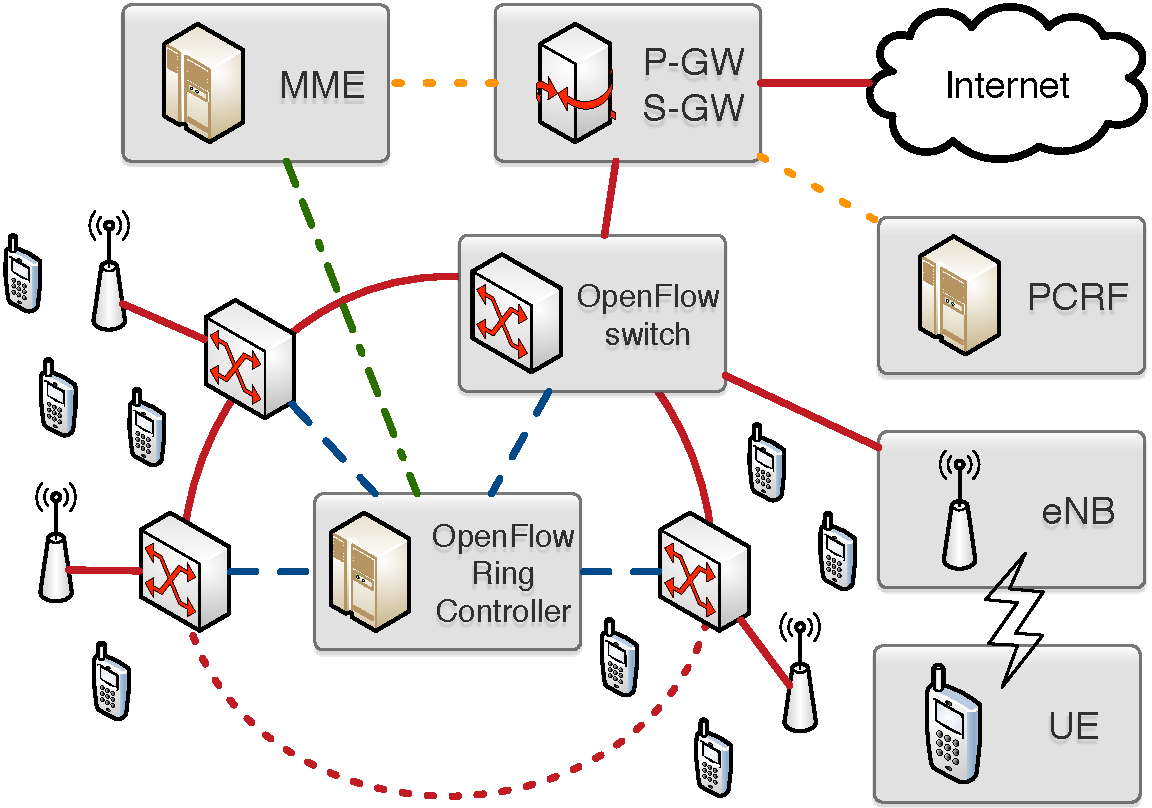
\includegraphics[width=.53\textwidth]{epcof-scenario}
    \label{fig:epcof-scenario}}
  \hfil \hspace{1cm}
    \subfloat[\acs{RAN} network topology.]
    {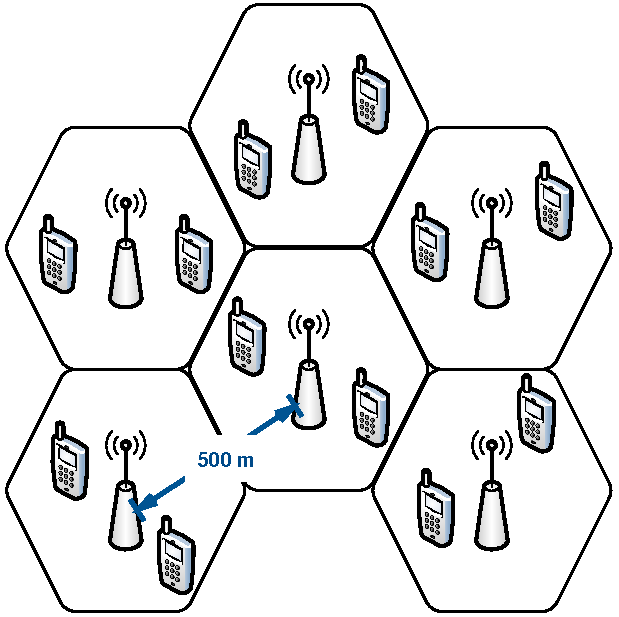
\includegraphics[width=.38\textwidth]{lte-scenario}
    \label{fig:lte-scenario}}
  \caption{\acs{SDN}-enabled \acs{LTE} network topology.}
  \label{fig:topology}
\end{figure}

Following the studies from \citet{Chundury2008} and \citet{Howard2011}, the
OpenFlow backhaul network is built over Ethernet technology, which is seen as
the most effective method to transport \ac{IP} packets and is the default
technology choice for a lower cost-per-bit as network scales to support large
capacity growth. The ring topology for backhaul network was chosen as most of
the legacy backhaul networks have a hub-spoke or ring access architecture.
Also, \citet{Nadiv2010} estate that the ring is one of the most efficient
topologies in terms of protection and is less costly than other topologies.
Nonetheless, it is possible to simulate different network topologies replacing
the connections between the switches.

\autoref{fig:lte-scenario} shows the \ac{RAN} topology, where each \ac{eNB}
covers an arbitrary number of active \acp{UE}. The \acp{eNB} are placed on a
hexagonal grid, 30 meters above the ground, and with an inter-site distance of
500 meters. \acp{UE} attached to each \ac{eNB} are scattered close to it, at
1.5 meters above the ground. \autoref{tab:lte-parameters} summarizes some of
the \ac{LENA} parameters that were adjusted in simulations. Any other \ac{LENA}
parameter not listed in the table was left on its default value.

\begin{table}[htb]
  \caption{\acs{LENA} simulation parameters.}
  \label{tab:lte-parameters}
  \centering
  \begin{tabular}{ll}
    \toprule
    \bfseries Parameter & \bfseries Value\\
    \midrule
    System frequency             & 2100\,MHz \\
    System bandwidth             & 20.0\,MHz \\
    \acs{eNB} transmission power & 46\,dBm \\
    \acs{UE} transmission power  & 18\,dBm \\
    \acs{SRS} periodicity        & 320\,ms \\
    Propagation model            & \texttt{OhBuildingsPropagationLossModel} \\
    MAC scheduler                & \texttt{CqaFfMacScheduler} \\
    \bottomrule
  \end{tabular}
\end{table}


%=============================================================================%
\subsection{OpenFlow \acs{EPC} controller}
\label{sec:controller}

The OpenFlow 1.3 controller base class was extended to implement a specialized
OpenFlow \ac{EPC} controller to manage the \ac{SDN}-enabled \ac{LTE} network.
The controller communicates with the \ac{MME} element in order to monitor for
bearer management functions in the \ac{NAS} protocol. In this way, the
controller can be aware of \ac{EPS} bearer context activation, modification,
and deactivation procedures. \autoref{subsec:mmecontroller} describes the
communication between the \ac{EPC} controller and the \ac{MME} element, while
Sections \ref{subsec:routing} through \ref{subsec:coexistence} describe the key
controller functionalities, along with some simulations to highlight the
benefits that can be achieved within this \ac{SDN}-enabled scenario.

%-----------------------------------------------------------------------------%
\subsubsection{Communication with the MME}
\label{subsec:mmecontroller}

This \ac{MME} element communicates with the \ac{EPC} controller to notify about
procedures related to bearer activation, modification or deactivation in the
\ac{NAS} protocol. A typical bearer establishment flow is shown in
\autoref{fig:bearer-establishment}, which also includes the communication with
the \ac{EPC} controller. Note that the modification and deactivation procedures
are similar to this.

\begin{figure}[b!]
  \centering
  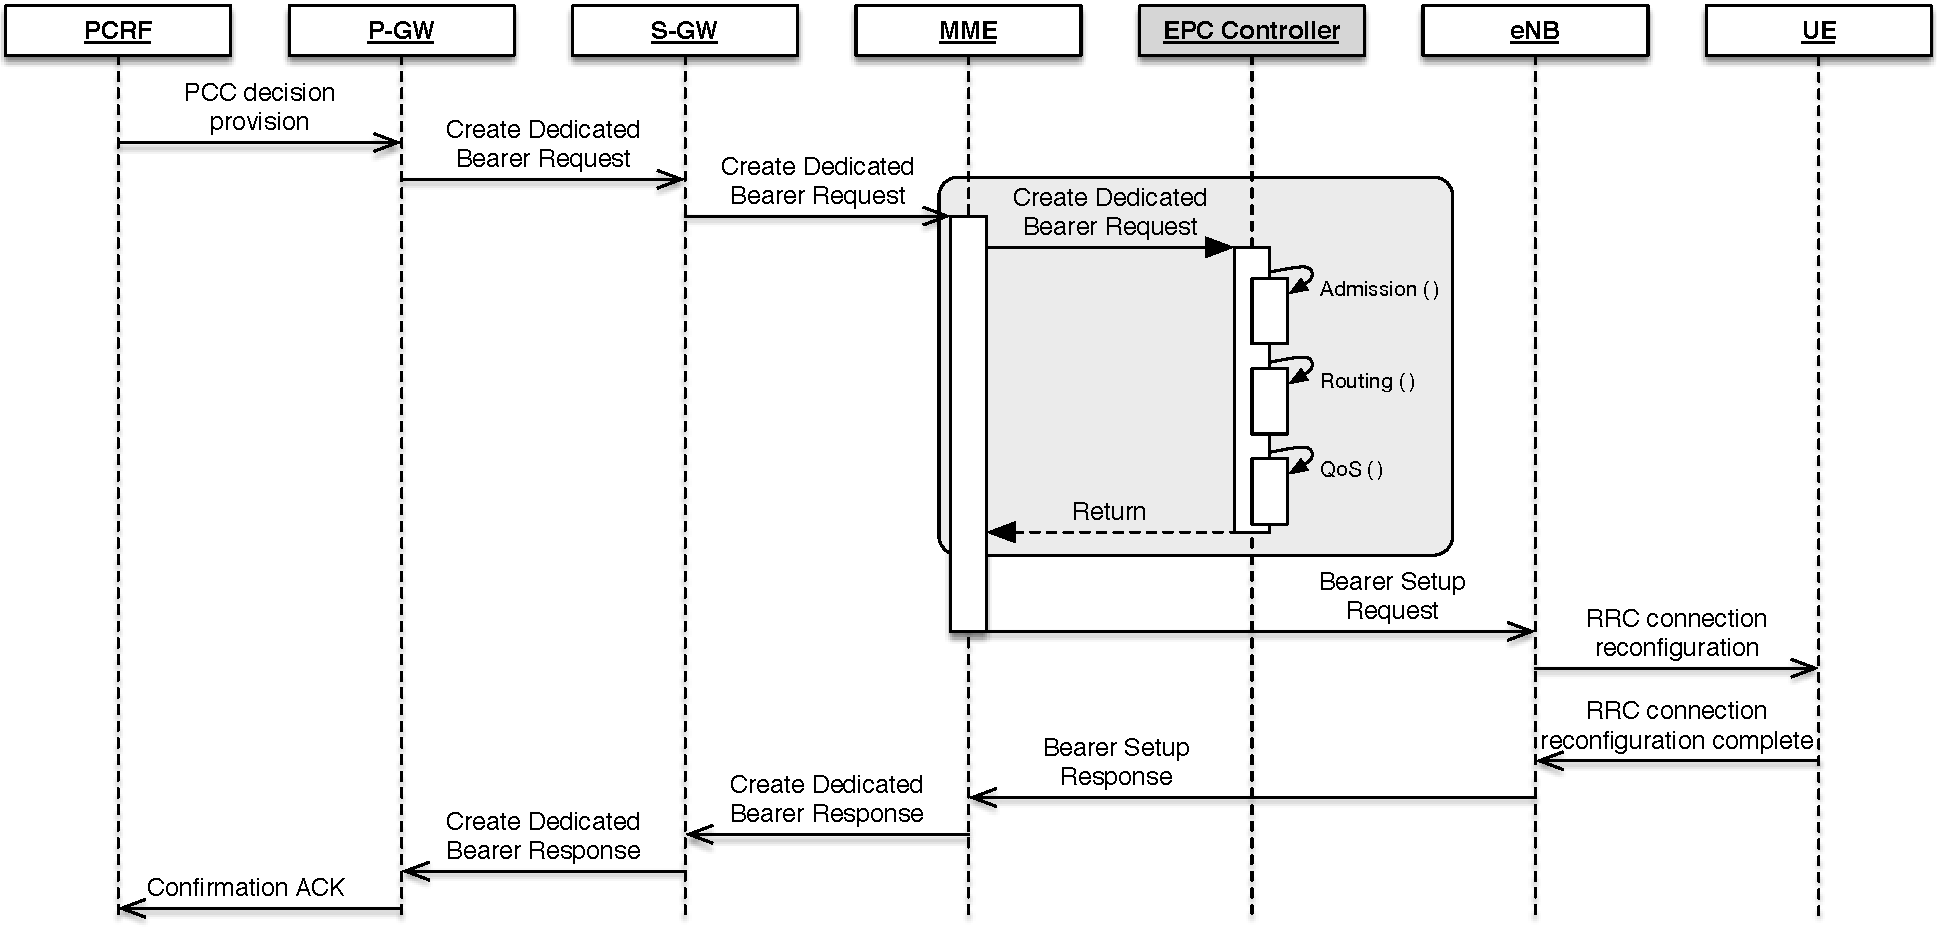
\includegraphics[width=\textwidth]{bearer-establishment}
  \caption{The message flow for an EPS bearer establishment procedure.}
  \label{fig:bearer-establishment}
\end{figure}

When an \ac{EPS} bearer is established, the \ac{PCRF} first sends a
\emph{\ac{PCC} Decision Provision} message indicating the required \ac{QoS} for
the bearer to the \ac{P-GW}. The \ac{P-GW} uses this \ac{QoS} policy to assign
the bearer-level \ac{QoS} parameters and sends a \emph{Create Dedicated
Bearer Request} message to the \ac{S-GW}, including the \ac{QoS} and the uplink
\ac{TFT} to be used in the \ac{UE}. The \ac{S-GW} forwards this message to the
\ac{MME}. At this point, the request message is forwarded to the \ac{EPC}
controller, which will trigger its internal mechanisms, including bearer
admission control, traffic routing and \ac{QoS} enforcement strategies. Once
these tasks have been successfully completed, the controller returns to the
\ac{MME}. At this point, the \ac{MME} continues with the establishment
procedure. It builds the \emph{Bearer Setup Request} message that it sent to
the \ac{eNB}. The \ac{eNB} maps the \ac{EPS} bearer \ac{QoS} to the radio
bearer \ac{QoS}. It then signals an \emph{\ac{RRC} Connection Reconfiguration}
message to the \ac{UE} to set up the radio bearer. The \emph{\ac{RRC}
Connection Reconfiguration} message contains all the configuration parameters
for the radio interface. This is mainly for the configuration of the Layer 2
(\ac{PDCP}, \ac{RLC} and \ac{MAC}) parameters, but also the Layer 1 parameters
required for the \ac{UE} to initialize the protocol stack. The following
messages are the corresponding response messages to confirm that the bearers
have been set up correctly.

%-----------------------------------------------------------------------------%
\subsubsection{Network traffic routing}
\label{subsec:routing}

Routing is the process of selecting paths in a network, and one of the greatest
advantages offered by the \ac{SDN} paradigm is the possibility to exploit
different routing strategies thanks to the centralized software controller.

The controller maintains a global view of the backhaul network, both in terms
of topology and bandwidth usage for each link. With this information, it is
possible to route traffic over the network using classical approaches like the
shortest path, based only on the source and destination \ac{IP} addresses.
Yet, more complex algorithms can be employed to route the traffic based on
requested bandwidth and \ac{QCI} requirements. Even sophisticated traffic
engineering strategies could be used in this scenario, like modeling the
network flow placement as linear programming problem and using a software to
find the optimal solution~\cite{Medhi2007}.

Once a new \ac{EPS} bearer context activation procedure is initiated in the
network, the controller searches for an acceptable route and install the match
rules into the switches before the traffic start. This is accomplished by the
communication between the controller and the \ac{MME} over the northbound
interface. Since the traffic in S1 interface is encapsulated within the
\ac{UDP}/\ac{IP}/\ac{GTP} protocol stack, the header fields exposed to the
OpenFlow matching procedures are those related to the tunnel between the
\ac{eNB} and \ac{S-GW}. To allow for a fine-grained per-flow routing, the
OpenFlow switches consider only the \ac{GTP} \ac{TEID} identifier to route the
traffic. In fact, this approach simplifies the match rules that are installed
into switches, which speed up the lookup processes.

For the ring backhaul network in the simulation scenario, the routing options
are reduced to the clockwise or counter-clockwise direction. In this way, the
controller was improved with two different routing policies: 
\begin{itemize}
  \item The \emph{Shortest Path Only} policy, which always route the traffic
  over the shortest path between the source and destination elements;

  \item The \emph{Shortest Path First} policy, which attempts to route the
  traffic over the shortest path first whenever possible, or send the traffic
  in the other direction when necessary. This approach exploits one of the
  advantages offered by the OpenFlow protocol: ease creation of selective
  routing paths for traffic between the same source and destination nodes.
\end{itemize}

Installed match rules are configured with idle timeout value that force rule
expiration due to traffic inactivity. The controller can also remove installed
rules after a bearer context deactivation procedure notified by the \ac{MME}.

%-----------------------------------------------------------------------------%
\subsubsection{Bearer admission control}
\label{subsec:admission}

Every time a new default or dedicated bearer is activated, modified or
deactivated in the \ac{LTE} network, the controller must be aware of the
procedure to install, update or remove \ac{TEID} routing rules. Besides routing
functionality, the \ac{EPC} controller also provides an admission control
mechanism for \ac{GBR} bearer activation and modification requests. To ensure
the associated \ac{QCI} requirements, \ac{GBR} bearers call for some bandwidth
allocation in the backhaul network. During the admission, the controller first
checks for the requested bandwidth over all links in the selected routing path.
When the requested bandwidth is available, the bearer activation/modification
proceeds. Otherwise, the controller can check for a new routing path (if
available), or block the bearer. When this happens, the \ac{MME} is notified
and the network aborts the context activation/modification procedure. The
proposed mechanism monitors only for \ac{GBR} bearer request. Once a bearer is
blocked, the \ac{UE} can optionally send the traffic over any Non-\ac{GBR}
bearer, with no \ac{QoS} guarantees.

Some simulations were performed to investigate how the traffic routing and the
bearer admission control mechanisms can work together in the \ac{SDN}-enabled
\ac{LTE} network. The backhaul ring network is set up with 100\,Mbps Ethernet
links, in configurations with 5 and 11 OpenFlow switches. The first switch is
always connected to the \ac{S-GW}, and there is one \ac{eNB} attached to each
remaining switch, which are numbered in the clockwise direction. Two load
distributions are also evaluated: the balanced load distribution, where the
\acp{UE} are equally distributed among all \acp{eNB}; and the unbalanced load
distribution, where 30\% of the \acp{UE} are connected to the \acp{eNB} in the
first half of the ring, while the other 70\% are connected to the \acp{eNB} in
the second half of the ring. This unbalanced configuration is intentionally
chosen to underline the benefits that can be achieved with the selective
routing offered by the OpenFlow. The bearer admission control mechanism is
configured to reserve up to 40\% of the link bandwidth for traffics over
\ac{GBR} bearers. 

\autoref{fig:block-avg} shows the average block ratio for \ac{GBR} bearer
requests, with 95\% confidence interval. It compares both traffic routing
policies (the \emph{shortest path only} and the \emph{shortest path first})
with an increasing number of \acp{UE} in four scenario configurations (4 and 10
\acp{eNB}, balanced and unbalanced loads). Figures \ref{fig:block_avg-4bal} and
\ref{fig:block_avg-10bal} show the average block ratio for scenarios with a
balanced load. There are no significant differences in the results for
scenarios with 4 and 10 \acp{eNB}. For both ring sizes, it is possible to
observe that the bandwidth requested by \ac{GBR} bearers cannot be satisfied
from 200 \acp{UE} onward, and the admission control mechanism starts blocking
some of the requests for both routing strategies. The \emph{shortest path
first} routing policy reduces the block ratio in average, still with no
statistical improvements withing the confidence interval. In turn, Figures
\ref{fig:block_avg-4unb} and \ref{fig:block_avg-10unb} show the average block
ratio for scenarios with an unbalanced load. Once again, there are no
significant differences in the results for scenarios with 4 and 10 \acp{eNB}.
However, the \emph{shortest path first} routing policy significantly reduces
the block ratio in these scenarios, lowering the average block ratio by about
3.7 percentage points after 250 \acp{UE}, and increasing by 33\% the number of
accepted bearers. 

\begin{figure}[htb]
  \centering
  \subfloat[4 eNBs and balanced load.]{
    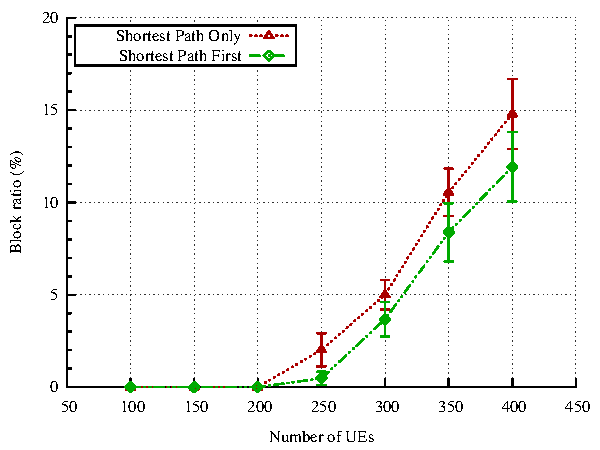
\includegraphics[width=.45\textwidth]{block_avg-4bal}
    \label{fig:block_avg-4bal}}
  \hfil
  \subfloat[10 eNBs and balanced load.]{
    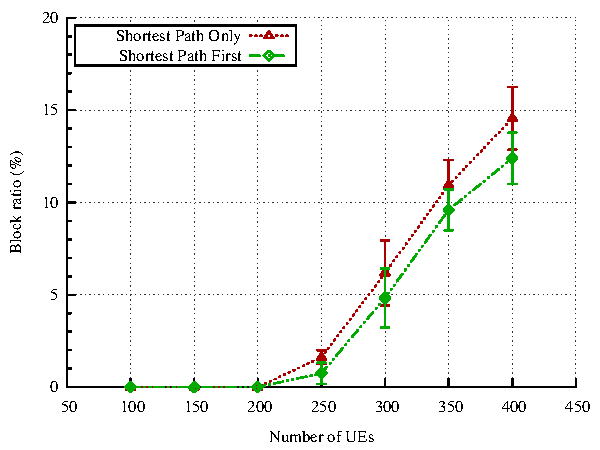
\includegraphics[width=.45\textwidth]{block_avg-10bal}
    \label{fig:block_avg-10bal}} \\
  \subfloat[4 eNBs and unbalanced load.]{
    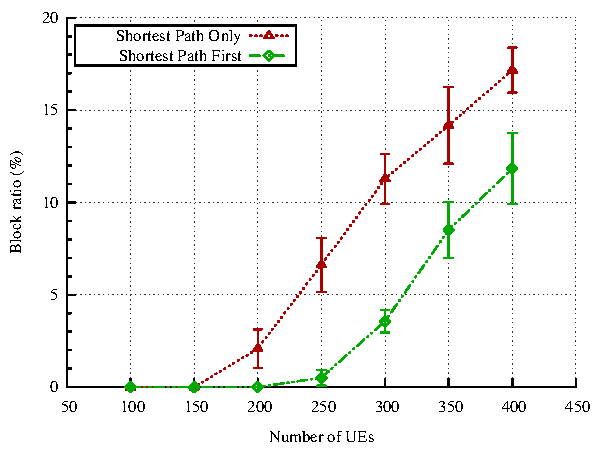
\includegraphics[width=.45\textwidth]{block_avg-4unb}
    \label{fig:block_avg-4unb}}
  \hfil
  \subfloat[10 eNBs and unbalanced load.]{
    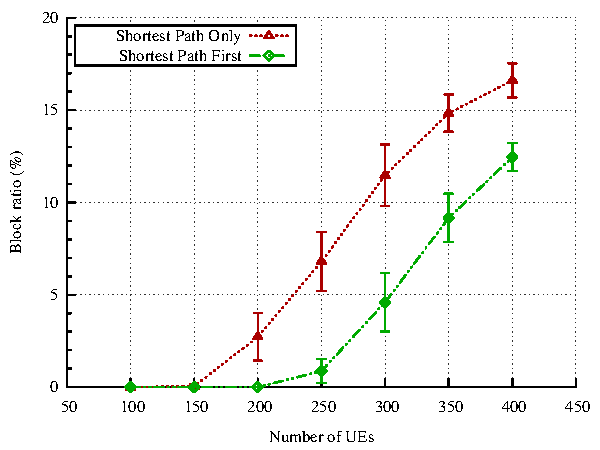
\includegraphics[width=.45\textwidth]{block_avg-10unb}
    \label{fig:block_avg-10unb}} 
  \caption{Average block ratio for \ac{GBR} bearer requests.}
  \label{fig:block-avg}
\end{figure}

\autoref{fig:enb-routing} validates previous results displaying the routing
path analysis for the simulations with 250 \acp{UE}. For each \ac{eNB}, it
shows the traffic distribution that are routed through the shortest path, the
inverted path, or that is blocked by the admission control mechanism. Figures
\ref{fig:enb-routing-4bal} and \ref{fig:enb-routing-10bal} bring the results
for balanced load scenarios. Note that the \emph{shortest path only} routing
policy blocks a small number of requests at all \acp{eNB}, while the
\emph{shortest path first} policy reduces the block ratio when exploiting some
available bandwidth over the inverted routing path. For the unbalanced load
scenarios, Figures \ref{fig:enb-routing-4unb} and \ref{fig:enb-routing-10unb}
confirm one of the benefits that can be achieved with the OpenFlow protocol:
the selective routing paths for traffics between the same source and
destination nodes. The first half of the ring has a few number of \acp{UE},
therefore, little traffic demand. The opposite occurs in the second half, where
the links cannot carry all the traffic. Thus, the \emph{shortest path only}
routing policy usage results in an odd block ratio distribution, penalizing
users on the overloaded side. This is solved with the \emph{routing path first}
policy, which redirects the exceeding traffic from the first half of the ring
to the other side, thus equalizing the block ratio among all \acp{eNB}.

\begin{figure}[htb]
  \centering
  \subfloat[4 eNBs and balanced load.]{
    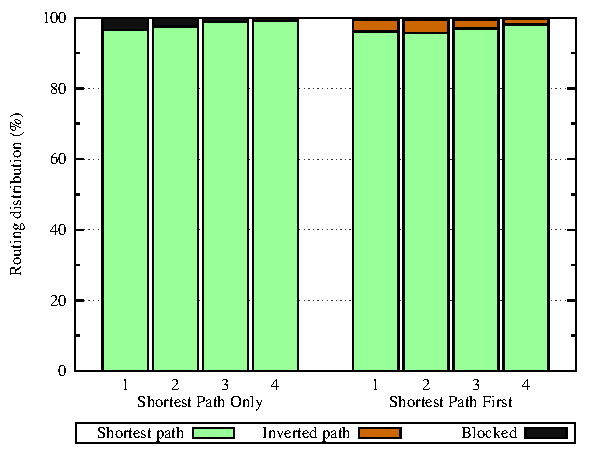
\includegraphics[width=.45\textwidth]{enb-routing-4bal-250}
    \label{fig:enb-routing-4bal}}
  \hfil
  \subfloat[10 eNBs and balanced load.]{
    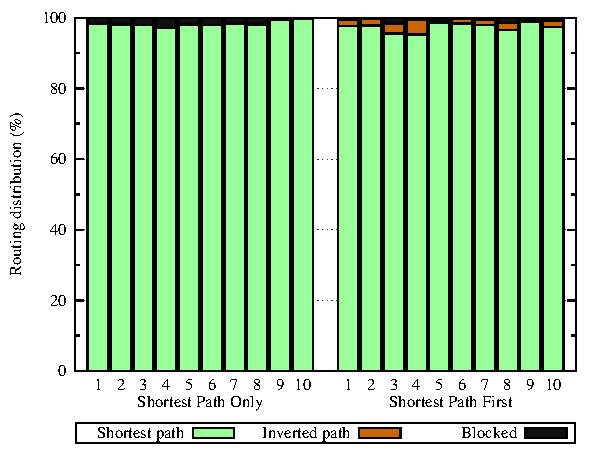
\includegraphics[width=.45\textwidth]{enb-routing-10bal-250}
    \label{fig:enb-routing-10bal}} \\
  \subfloat[4 eNBs and unbalanced load.]{
    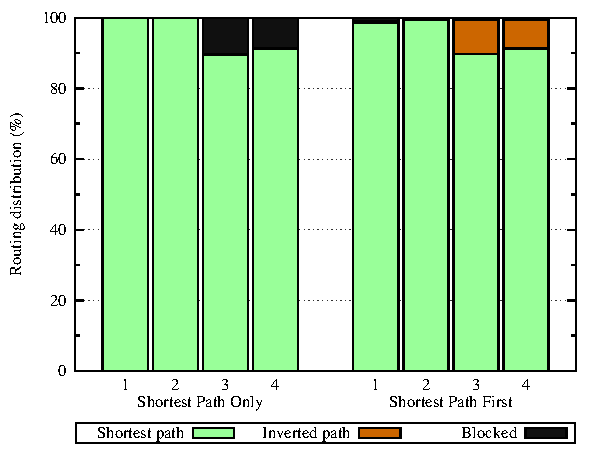
\includegraphics[width=.45\textwidth]{enb-routing-4unb-250}
    \label{fig:enb-routing-4unb}}
  \hfil
  \subfloat[10 eNBsand unbalanced load.]{
    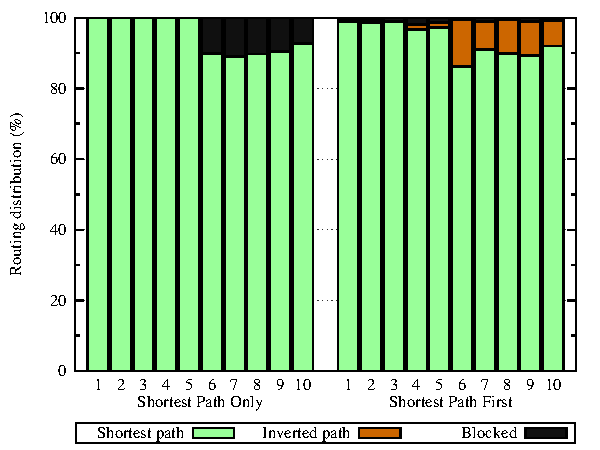
\includegraphics[width=.45\textwidth]{enb-routing-10unb-250}
    \label{fig:enb-routing-10unb}} 
  \caption{Routing distribution for \ac{GBR} bearer requests.}
  \label{fig:enb-routing}
\end{figure}

%-----------------------------------------------------------------------------%
\subsubsection{\acs{LTE} \acs{QoS} realization}
\label{subsec:coexistence}

The available resources in the \ac{LTE} backhaul infrastructure are physically
shared among all \ac{EPS} bearers, regardless of whether its resource type is
\ac{GBR} or Non-\ac{GBR}. Nonetheless, the network is supposed to allocate the
requested bandwidth along \ac{GTP} tunnel path for all \ac{GBR} bearers
accepted by the network admission control function. The actual resource
allocation and traffic management is not specified by \ac{3GPP} standards and
are left up to vendors and network operators, which can establish policies and
set up equipment accordingly.

The backhaul infrastructure can be built using different technologies with
layer 2 (L2) or layer 3 (L3) capabilities. \citet{Howard2011} argues that many
mobile operators and backhaul network providers want to keep their access and
aggregation networks simpler by avoiding L3 protocols, with no dynamic routing
and signaling across the backhaul to the cell site. When there are no routers,
the \ac{LTE} \ac{QoS} mechanisms can be implemented at \ac{MAC} layer as
\acs{IEEE} 802.1q \acp{VLAN} with \acs{IEEE} 802.1p traffic class
priorities~\cite{8021d2004}. According to \citet{Kempf2012a}, another commonly
used approach is the \ac{MPLS}~\cite{mpls} at layer~2.5. Both \ac{VLAN} and
\ac{MPLS} approaches demand frame encapsulation with an extra header.

However, as \ac{LTE} is \ac{IP}-based, it can leverage differentiated services
for classifying and managing network traffic and providing \ac{QoS} on a
per-hop basis. The most common technique used is Differentiated Services
(DiffServ)~\cite{rfc2474}, which uses the 6-bit \ac{DSCP} field in the \ac{IP}
header for traffic management. In \ac{LTE}, the \ac{QCI} can be directly mapped
to \ac{DSCP}. The basic classes defined by DiffServ are the \emph{default},
\emph{expedited forwarding}, and \emph{assured forwarding}. Of these, expedited
forwarding is used for strict priority traffic (e.g., video and voice), assured
forwarding is used for business differentiation (e.g., weighted-fair priority),
and the default is for best-effort traffic~\cite{Sandvine2014}. Backhaul
network nodes can implement queue management schemes and scheduling algorithms
for uplink and downlink traffic. In the backhaul network, the \ac{EPS} bearer
is not visible; and hence, these algorithms determine the per-hop traffic
forwarding treatment of each individual packet, based on the \ac{DSCP}
value~\cite{Ekstrom2009}.

With OpenFlow switches, it is possible to take advantage offered by L3 DiffServ
over the backhaul network. An OpenFlow switch provides limited \ac{QoS} support
through a simple queuing mechanism. One or more queues can attach to a port
and be used to map flow entries on it. The \ac{DSCP} field can map flow entries
to a specific queue, and packets will be treated according to the
configurations of that queue~\cite{ofs151}. 
% Also, the controller can provide fast optimized routing and improved user
% experience.

Some simulations were performed to investigate the resource sharing impact
between \ac{GBR} and Non-\ac{GBR} traffic, and how the OpenFlow protocol can be
used to implement the \ac{LTE} \ac{QoS} mechanisms. The backhaul ring network
is set up with 100\,Mbps Ethernet links with 10 OpenFlow switches. There is one
\ac{eNB} attached to each switch (except for the one connected to the gateway),
and \acp{UE} are equally distributed among them. The bearer admission control
mechanism is configured to reserve up to 40\% of the link bandwidth.  The
routing policy in use is the \emph{shortest path first}, which exploits
selective routing. All applications are enabled during the simulation.

The first simulations were used to investigate how the \ac{GBR} traffic can be
affected by Non-\ac{GBR} traffic in a backhaul network with shared bandwidth
resources and no traffic management. The bearer admission control still checks
for available bandwidth and blocks requests that exceed the allowed limit, but
there is no other mechanism in the backhaul network to assure resource
reservation. All packets traversing the network are handled in the same way,
over the same single output queues. \autoref{fig:coex-prob} shows the \ac{GBR}
traffic throughput and packet loss ratio for different numbers of \acp{UE} and
fixed network capacity. These values represent the aggregated results for
traffic on both links adjacent to gateway switch.

\begin{figure}[t!]
  \centering
    \subfloat[Traffic throughput and \acs{GBR} reserved bandwidth.]
    {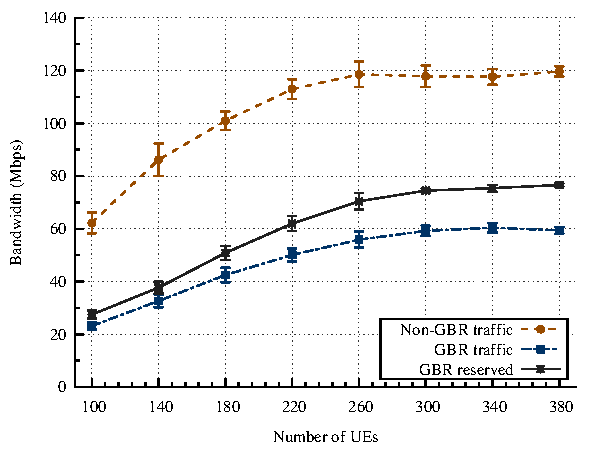
\includegraphics[width=.45\textwidth]{coex-problem-thp}
    \label{fig:coex-prob-thp}}
  \hfil
    \subfloat[Packet loss ratio at queues.]
    {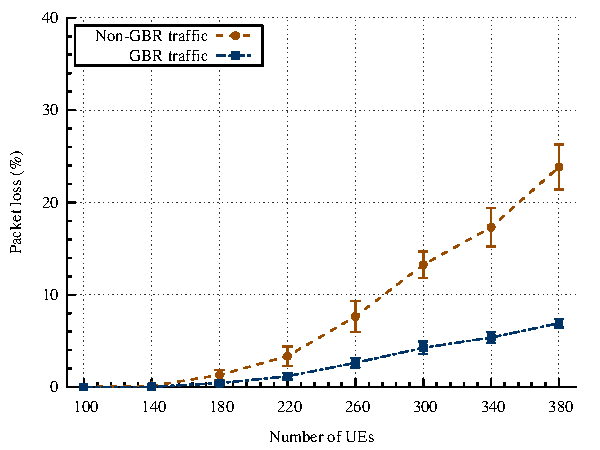
\includegraphics[width=.45\textwidth]{coex-problem-loss}
    \label{fig:coex-prob-loss}}
  \caption{\acs{GBR}/Non-\acs{GBR} traffic analysis
           for the coexistence problem.}
  \label{fig:coex-prob}
\end{figure}

As network traffic load grows, it is possible to observe an increasing gap
between the \ac{GBR} bandwidth reserved by the bearer admission control and the
actual \ac{GBR} traffic throughput (\autoref{fig:coex-prob-thp}), mainly caused
by a large \ac{GBR} packet loss ratio (\autoref{fig:coex-prob-loss}). This
increasing loss ratio is caused by overflowing queue buffers. In fact, when
there is no available bandwidth to carry all network traffic, only Non-\ac{GBR}
packets should be discarded, as services over GBR bearers can assume that
congestion-related packet losses will not occur.

To overcome this situation, the proposed \emph{coexistence mechanism} has to
keep both \ac{GBR} and Non-\ac{GBR} traffic within its allowed bandwidth. To
enable for traffic separation and fast classification in the backhaul network,
the OpenFlow switches connected to the gateway or to the \ac{eNB} implement a
\ac{QCI} to \ac{DSCP} mapping function. The purpose of this function is to make
a translation from bearer-level \ac{QoS} (\ac{QCI}) to transport-level \ac{QoS}
(\ac{DSCP}). Using this function, packets on a bearer associated with a
specific \ac{QCI} are marked with a specific \ac{DSCP} for forwarding in the
backhaul network~\cite{Astudillo2014b, Ekstrom2009}. The \ac{QCI} to \ac{DSCP}
mapping can be performed based on network operator policies, and here is
implemented as indicated at \autoref{tab:dscp}.

\begin{table}[b!]
  \renewcommand{\arraystretch}{1.3}
  \caption{\acs{QCI} to \acs{DSCP} mapping table.}
  \label{tab:dscp}
  \centering
  \begin{tabular}{ll}
    \toprule
    \bfseries \acs{LTE} \acs{QCI} & \bfseries \acs{IP} \acs{DSCP} \\
    \midrule
    1       & 44 (Voice admit)            \\
    2       & 12 (Assured forwarding 13)  \\
    3       & 18 (Assured forwarding 21)  \\
    4       & 18 (Assured forwarding 21)  \\
    5 -- 9  & 00 (Default / best effort)  \\
    \bottomrule
  \end{tabular}
\end{table}

As packets traversing the backhaul network are encapsulated by \ac{GTP}
protocol, only the outermost \ac{IP} header (from the \ac{GTP} encapsulation)
is marked with the mapped \ac{DSCP} value. The \ac{DSCP}, together with
\ac{GTP} \ac{TEID} values, are used by the OpenFlow switches to identify the
\ac{EPS} bearer and properly route the traffic over the network, applying the
correct forwarding treatment.

To limit traffic throughput up to the allowed bandwidth, the OpenFlow
\emph{meter table} is used to measure and control the rate of packets. The
meter triggers a meter band if the packet rate or byte rate passing through the
meter exceed a predefined threshold. Two types of meters are in use:
\begin{enumerate}
  \item \emph{\ac{GBR} per-flow meter}, which is used to limit the \ac{GBR}
  bearer throughput up to the \ac{GBR} \ac{MBR} value. These meters are
  installed together with the \ac{DSCP} marking process.

  \item \emph{Non-\ac{GBR} coexistence meter}, which is used to limit the
  aggregated Non-\ac{GBR} traffic throughput over each link, effectively
  reserving the bandwidth for active \ac{GBR} bearers. These bearers are
  regularly updated by the bearer admission control over the routing path
  selected for newly accepted bearers.
\end{enumerate}

\autoref{fig:coex} shows some simulation results for the proposed coexistence
mechanism. It is possible to observe that Non-\ac{GBR} coexistence meters can
properly limit the Non-\ac{GBR} traffic, allowing \ac{GBR} traffic to use the
reserved bandwidth. \autoref{fig:coex-thp} shows the traffic throughput for
both resource types while \autoref{fig:coex-thp-comp} highlights the \ac{GBR}
throughput with and without the coexistence mechanism (in comparison to
\autoref{fig:coex-prob-thp}). Also, the packet loss ratio at queues
(\autoref{fig:coex-loss}) is reduced for both traffics, but a new packet drop
ratio is introduced by the use of OpenFlow meters (\autoref{fig:coex-drops}).
Here, it is possible to observe the constant \ac{GBR} drop ratio triggered by
the per-flow meters limiting the individual \ac{EPS} bearer throughput, and an
increasing drop ratio for Non-\ac{GBR} traffic due to Non-\ac{GBR} coexistence
meters.

An additional improvement to the coexistence mechanism is the use of OpenFlow
queue support to better treat \ac{VoIP} traffic over the backhaul network. To
provide the required voice quality, \ac{QoS} capability must be added to the
traditional data-only network. In an environment of mixed real-time and bulk
traffic, it is natural to use priority queuing to give the real-time traffic
priority service. This works quite well as long as the real-time traffic is
less than some fixed fraction of the total~\cite{Dordal2015, rfc3246}.

A new group of simulations was performed, now including a second high-priority
queue at each OpenFlow output port. Only \ac{VoIP} traffic (identified by the
\ac{DSCP} unique value) is mapped to this new queue. \autoref{fig:coex-voip}
compares both delay and jitter for \ac{VoIP} traffic over the backhaul network,
considering the first simulations without traffic management (Coex. OFF), the
second group simulations with coexistence mechanism (Coex. ON), and this third
group of simulations with the new \ac{VoIP} queuing mechanism (VoIP queues).
The use of high-priority queues for \ac{VoIP} traffic results in a constant
average delay and jitter for this type of traffic, regardless how congested the
network is. Also, it is possible to observe that, even without exclusive
queues, the coexistence mechanism also improved network average delay, with a
small jitter increase for high load scenarios.

\begin{figure}[p]
  \centering
    \subfloat[Traffic throughput and \acs{GBR} reserved bandwidth.]
    {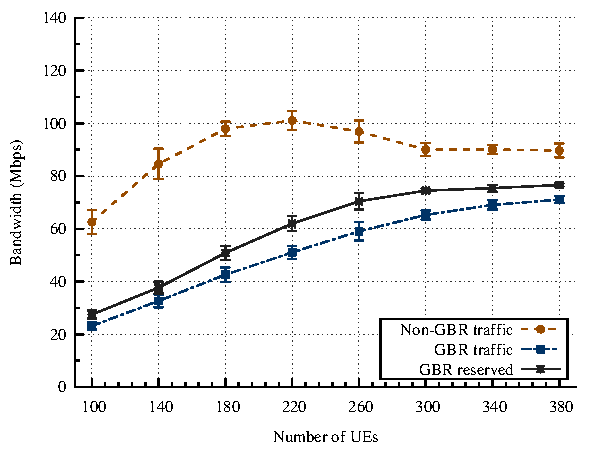
\includegraphics[width=.45\textwidth]{coex-thp}
    \label{fig:coex-thp}}
  \hfil
    \subfloat[\acs{GBR} traffic throughput comparison.]
    {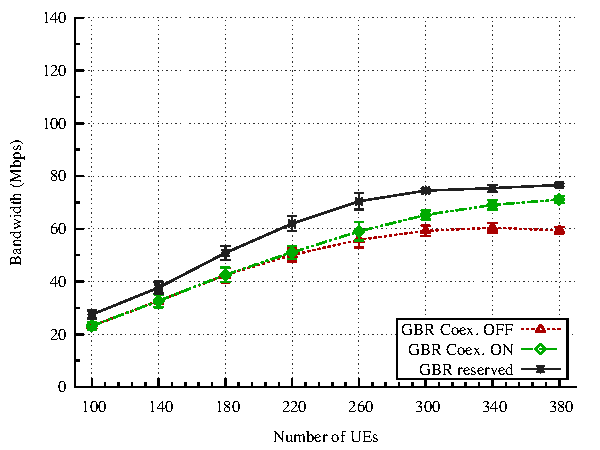
\includegraphics[width=.45\textwidth]{coex-thp-comp}
    \label{fig:coex-thp-comp}}
  \hfil
    \subfloat[Packet loss ratio at queues.]
    {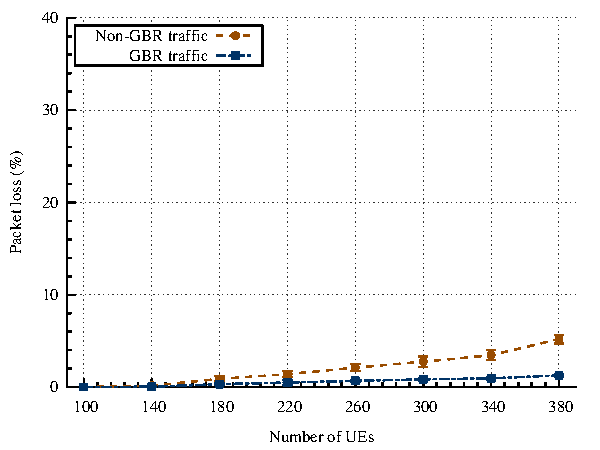
\includegraphics[width=.45\textwidth]{coex-loss}
    \label{fig:coex-loss}}
  \hfil
    \subfloat[Packet drop ratio by OpenFlow meters.]
    {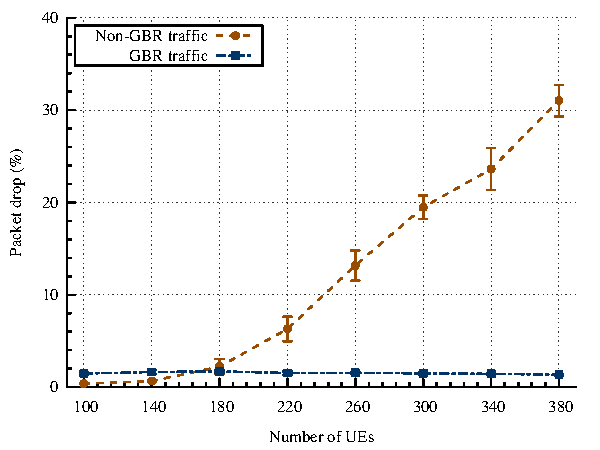
\includegraphics[width=.45\textwidth]{coex-drops}
    \label{fig:coex-drops}}
  \caption{\acs{GBR}/Non-\acs{GBR} traffic coexistence with OpenFlow.}
  \label{fig:coex}
  
  \vspace*{\floatsep}
  
  \centering
    \subfloat[\acs{VoIP} delay comparison.]
    {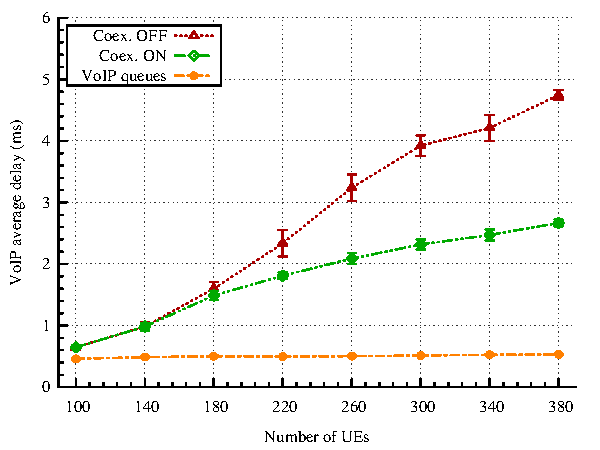
\includegraphics[width=.45\textwidth]{coex-voip-delay}
    \label{fig:voip-delay}}
  \hfil
    \subfloat[\acs{VoIP} jitter comparison.]
    {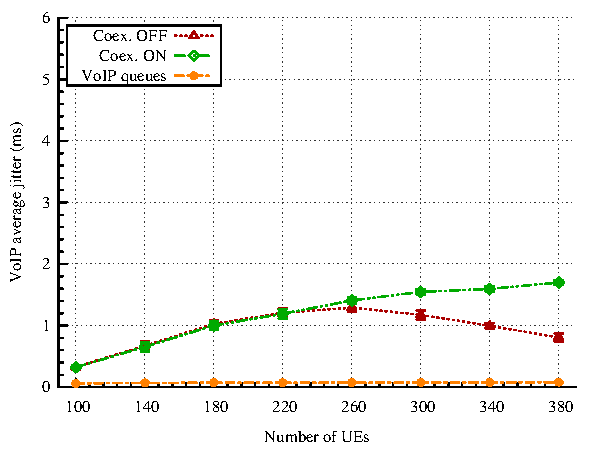
\includegraphics[width=.45\textwidth]{coex-voip-jitter}
    \label{fig:voip-jitter}}
  \caption{\acs{VoIP} traffic analysis.}
  \label{fig:coex-voip}
\end{figure}
